\documentclass[border=4pt]{standalone}

\usepackage{amsmath}
\usepackage{tikz}
\usepackage{mathdots}
\usepackage{yhmath}
\usepackage{cancel}
\usepackage{color}
\usepackage{siunitx}
\usepackage{array}
\usepackage{multirow}
\usepackage{amssymb}
\usepackage{gensymb}
\usepackage{tabularx}
\usepackage{booktabs}
\usetikzlibrary{fadings}
\usetikzlibrary{patterns}


\begin{document}
 


\tikzset{every picture/.style={line width=0.75pt}} %set default line width to 0.75pt        

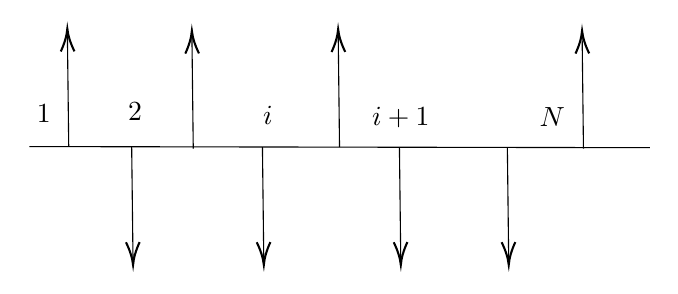
\begin{tikzpicture}[x=0.75pt,y=0.75pt,yscale=-1,xscale=1]
%uncomment if require: \path (0,300); %set diagram left start at 0, and has height of 300

%Straight Lines [id:da4625837896137932] 
\draw    (111,170) -- (409.95,170.54) ;


%Straight Lines [id:da2761971380946687] 
\draw    (130,170) -- (129.35,115.22) ;
\draw [shift={(129.33,113.22)}, rotate = 449.32] [color={rgb, 255:red, 0; green, 0; blue, 0 }  ][line width=0.75]    (10.93,-3.29) .. controls (6.95,-1.4) and (3.31,-0.3) .. (0,0) .. controls (3.31,0.3) and (6.95,1.4) .. (10.93,3.29)   ;

%Straight Lines [id:da5742772653407224] 
\draw    (378,171) -- (377.35,116.22) ;
\draw [shift={(377.33,114.22)}, rotate = 449.32] [color={rgb, 255:red, 0; green, 0; blue, 0 }  ][line width=0.75]    (10.93,-3.29) .. controls (6.95,-1.4) and (3.31,-0.3) .. (0,0) .. controls (3.31,0.3) and (6.95,1.4) .. (10.93,3.29)   ;

%Straight Lines [id:da6503647597755311] 
\draw    (260.47,170.27) -- (259.83,115.49) ;
\draw [shift={(259.8,113.49)}, rotate = 449.32] [color={rgb, 255:red, 0; green, 0; blue, 0 }  ][line width=0.75]    (10.93,-3.29) .. controls (6.95,-1.4) and (3.31,-0.3) .. (0,0) .. controls (3.31,0.3) and (6.95,1.4) .. (10.93,3.29)   ;

%Straight Lines [id:da44830391865347163] 
\draw    (190,171) -- (189.35,116.22) ;
\draw [shift={(189.33,114.22)}, rotate = 449.32] [color={rgb, 255:red, 0; green, 0; blue, 0 }  ][line width=0.75]    (10.93,-3.29) .. controls (6.95,-1.4) and (3.31,-0.3) .. (0,0) .. controls (3.31,0.3) and (6.95,1.4) .. (10.93,3.29)   ;

%Straight Lines [id:da5398436448074991] 
\draw    (160.98,225) -- (160.56,189.45) -- (160.33,170.22) ;

\draw [shift={(161,227)}, rotate = 269.32] [color={rgb, 255:red, 0; green, 0; blue, 0 }  ][line width=0.75]    (10.93,-3.29) .. controls (6.95,-1.4) and (3.31,-0.3) .. (0,0) .. controls (3.31,0.3) and (6.95,1.4) .. (10.93,3.29)   ;
%Straight Lines [id:da04929405586601365] 
\draw    (289.98,225) -- (289.56,189.45) -- (289.33,170.22) ;

\draw [shift={(290,227)}, rotate = 269.32] [color={rgb, 255:red, 0; green, 0; blue, 0 }  ][line width=0.75]    (10.93,-3.29) .. controls (6.95,-1.4) and (3.31,-0.3) .. (0,0) .. controls (3.31,0.3) and (6.95,1.4) .. (10.93,3.29)   ;
%Straight Lines [id:da8000252480392469] 
\draw    (223.98,225) -- (223.56,189.45) -- (223.33,170.22) ;

\draw [shift={(224,227)}, rotate = 269.32] [color={rgb, 255:red, 0; green, 0; blue, 0 }  ][line width=0.75]    (10.93,-3.29) .. controls (6.95,-1.4) and (3.31,-0.3) .. (0,0) .. controls (3.31,0.3) and (6.95,1.4) .. (10.93,3.29)   ;
%Straight Lines [id:da5700920925616243] 
\draw    (341.98,225) -- (341.56,189.45) -- (341.33,170.22) ;

\draw [shift={(342,227)}, rotate = 269.32] [color={rgb, 255:red, 0; green, 0; blue, 0 }  ][line width=0.75]    (10.93,-3.29) .. controls (6.95,-1.4) and (3.31,-0.3) .. (0,0) .. controls (3.31,0.3) and (6.95,1.4) .. (10.93,3.29)   ;

% Text Node
\draw (118,154) node   {$1$};
% Text Node
\draw (162,153) node   {$2$};
% Text Node
\draw (226,155) node   {$i$};
% Text Node
\draw (290,156) node   {$i+1$};
% Text Node
\draw (363,156) node   {$N$};


\end{tikzpicture}

\end{document}
